% Figures for the Module 4 pen-and-paper sheet, shared with its answer key.
% Kept in their own file because the key draws exactly the same grids with the
% bars and the dots put in -- an answer to a question about a chart has to be a
% chart, and a column of counts cannot show a student the shape they were meant
% to see.
%
% Needs tikz and the colour pltblue, both of which the including file sets up.
% ---------------------------------------------------------------------------
\tikzset{
  axisline/.style = {line width=0.9pt, black!75, line cap=round},
  gridline/.style = {line width=0.5pt, black!16},
  binsep/.style   = {line width=0.5pt, black!28, dash pattern=on 2pt off 2pt},
  barstyle/.style = {line width=1.1pt, draw=pltblue!72!black, fill=pltblue!20},
  ccdfdot/.style  = {circle, fill=pltblue!72!black, inner sep=0pt,
                     minimum size=6pt},
  marker/.style   = {line width=1.6pt, pltblue!72!black, line cap=round},
  tlab/.style     = {font=\small},
  slab/.style     = {font=\footnotesize},
}

% ---------------------------------------------------------------------------
% Part 1: four pairs of shapes. The big one is 4x the small one in the measure
% named under each pair -- except the cube, which is 8x. That mismatch is the
% whole question: the eye reads all four pairs as roughly the same jump.
% ---------------------------------------------------------------------------
\newcommand{\sizeline}{%
\begin{tikzpicture}[xkcd, line width=1.1pt]
  \draw (0,0.75) -- (1,0.75);
  \draw (0,0) -- (4,0);
\end{tikzpicture}}

\newcommand{\sizesquare}{%
\begin{tikzpicture}[xkcd, line width=1.1pt]
  \draw (0,0) rectangle (1,1);
  \draw (1.7,0) rectangle (3.7,2);
\end{tikzpicture}}

\newcommand{\sizecircle}{%
\begin{tikzpicture}[xkcd, line width=1.1pt]
  \draw (0,1) circle (0.5cm);
  \draw (2.2,1) circle (1cm);
\end{tikzpicture}}

\newcommand{\sizecube}{%
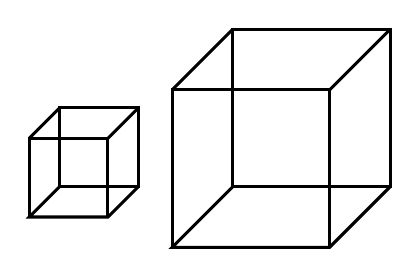
\begin{tikzpicture}[line width=1.1pt]
  \draw (0,0,0) -- (1,0,0) -- (1,1,0) -- (0,1,0) -- cycle;
  \draw (0,0,0) -- (0,0,1) -- (1,0,1) -- (1,0,0);
  \draw (1,0,1) -- (1,1,1) -- (0,1,1) -- (0,0,1);
  \draw (1,1,0) -- (1,1,1);
  \draw (0,1,0) -- (0,1,1);
  \begin{scope}[xshift=2.2cm, scale=2]
  \draw (0,0,0) -- (1,0,0) -- (1,1,0) -- (0,1,0) -- cycle;
  \draw (0,0,0) -- (0,0,1) -- (1,0,1) -- (1,0,0);
  \draw (1,0,1) -- (1,1,1) -- (0,1,1) -- (0,0,1);
  \draw (1,1,0) -- (1,1,1);
  \draw (0,1,0) -- (0,1,1);
  \end{scope}
\end{tikzpicture}}

% ---------------------------------------------------------------------------
% Part 2: the equal-bin chart. Five bins five hours wide, from 0 to 25.
% The y axis reaches 16 because one bin holds sixteen of the twenty people,
% which is the point of the picture.
% ---------------------------------------------------------------------------
\newcommand{\linbar}[3]{\draw[barstyle] (#1,0) rectangle (#2,#3);}

\newcommand{\linhist}[1]{%
\begin{tikzpicture}[x=0.47cm, y=0.36cm]
  \foreach \y in {4,8,12,16} \draw[gridline] (0,\y) -- (25.6,\y);
  \foreach \x in {5,10,15,20} \draw[binsep] (\x,0) -- (\x,17.5);
  #1
  \draw[axisline] (0,0) -- (26.4,0);
  \draw[axisline] (0,0) -- (0,17.5);
  \foreach \x in {0,5,10,15,20,25} {
    \draw[axisline] (\x,0) -- ++(0,-0.16cm);
    \node[tlab, below] at (\x,-0.55) {\x};}
  \foreach \y in {0,4,8,12,16} {
    \draw[axisline] (0,\y) -- ++(-0.16cm,0);
    \node[tlab, left] at (-0.4,\y) {\y};}
  \node[tlab] at (13,-3.7) {hours watched last week};
  \node[tlab, rotate=90] at (-3.4,8.75) {people};
\end{tikzpicture}}

% ---------------------------------------------------------------------------
% Part 3: the doubling-bin chart. Six bins, each drawn the same width, which
% is what a log axis is. Slot i runs from i to i+1.
% ---------------------------------------------------------------------------
\newcommand{\logbar}[2]{\draw[barstyle] (#1,0) rectangle (#1+1,#2);}

\newcommand{\loghist}[1]{%
\begin{tikzpicture}[x=1.78cm, y=0.45cm]
  \foreach \y in {2,4,6,8} \draw[gridline] (0,\y) -- (6.1,\y);
  \foreach \x in {1,2,3,4,5} \draw[binsep] (\x,0) -- (\x,9.3);
  #1
  \draw[axisline] (0,0) -- (6.3,0);
  \draw[axisline] (0,0) -- (0,9.3);
  \foreach \y in {0,2,4,6,8} {
    \draw[axisline] (0,\y) -- ++(-0.10cm,0);
    \node[tlab, left] at (-0.062,\y) {\y};}
  \foreach \x/\lab in {0/{0--1}, 1/{1--2}, 2/{2--4}, 3/{4--8},
                       4/{8--16}, 5/{16--32}} {
    \node[slab] at (\x+0.5,-0.95) {\lab};}
  \node[tlab] at (3,-2.5) {hours watched last week};
  \node[tlab, rotate=90] at (-0.60,4.65) {people};
\end{tikzpicture}}

% ---------------------------------------------------------------------------
% Part 3: the two rulers. Both are the same length on paper. The top one
% spreads 0 to 32 evenly; on the bottom one every step doubles.
% #1 is whatever gets marked on them.
% ---------------------------------------------------------------------------
\newcommand{\rulers}[1]{%
\begin{tikzpicture}[y=1cm]
  % Top: even spacing, 0 to 32 across 12cm.
  \draw[axisline] (0,3.6) -- (12.4,3.6);
  \foreach \n in {0,4,8,12,16,20,24,28,32} {
    \draw[axisline] (\n*0.375,3.6) -- ++(0,-0.24);
    \node[tlab, below] at (\n*0.375,3.36) {\n};}
  \node[tlab, anchor=west] at (0,4.65) {\bfseries Ruler A \normalfont ---
    every step adds 4};
  % Bottom: doubling, 1 to 32 across the same 12cm.
  \draw[axisline] (0,0) -- (12.4,0);
  \foreach \n/\p in {1/0, 2/1, 4/2, 8/3, 16/4, 32/5} {
    \draw[axisline] (\p*2.4,0) -- ++(0,-0.24);
    \node[tlab, below] at (\p*2.4,-0.24) {\n};}
  \node[tlab, anchor=west] at (0,0.5) {\bfseries Ruler B \normalfont ---
    every step doubles};
  #1
\end{tikzpicture}}

% ---------------------------------------------------------------------------
% Part 4: the doubling grid the five counted fractions are plotted on. Both
% rulers double, so five points that halve each time land on a straight line.
% Slot i on x is 1,2,4,8,16; slot j on y is 0.05,0.1,0.2,0.4,0.8.
% ---------------------------------------------------------------------------
\newcommand{\ccdfgrid}[1]{%
\begin{tikzpicture}[x=2.35cm, y=1.72cm]
  \foreach \j in {0,1,2,3,4} \draw[gridline] (0,\j) -- (4.3,\j);
  \foreach \i in {0,1,2,3,4} \draw[gridline] (\i,-0.3) -- (\i,4.3);
  #1
  % The axes sit clear of the lowest gridline, so the point that lands on
  % 0.05 is not drawn half underneath the axis.
  \draw[axisline] (-0.12,-0.3) -- (4.4,-0.3);
  \draw[axisline] (0,-0.42) -- (0,4.4);
  \foreach \i/\lab in {0/1, 1/2, 2/4, 3/8, 4/16} {
    \draw[axisline] (\i,-0.3) -- ++(0,-0.10cm);
    \node[tlab, below] at (\i,-0.385) {\lab};}
  \foreach \j/\lab in {0/{0.05}, 1/{0.1}, 2/{0.2}, 3/{0.4}, 4/{0.8}} {
    \draw[axisline] (0,\j) -- ++(-0.10cm,0);
    \node[tlab, left] at (-0.043,\j) {\lab};}
  \node[tlab] at (2,-1.15) {$k$ hours};
  \node[tlab, rotate=90] at (-0.66,1.85)
    {fraction watching more than $k$};
\end{tikzpicture}}

% ---------------------------------------------------------------------------
% The worked charts, used by solutions.tex only. They live here so that the
% blank grid and the filled one can never drift apart.
% ---------------------------------------------------------------------------
% Part 2: sixteen people in the first bin, three in the second, none in the
% next two, one at the far right.
\newcommand{\linsol}{%
  \linbar{0}{5}{16}\linbar{5}{10}{3}\linbar{20}{25}{1}}

% Part 3: 4, 8, 4, 2, 1, 1 -- every bar visible, and after the peak each one
% is half the one before.
\newcommand{\logsol}{%
  \logbar{0}{4}\logbar{1}{8}\logbar{2}{4}\logbar{3}{2}\logbar{4}{1}%
  \logbar{5}{1}}

% Part 3: where 5 lands on each ruler. On Ruler A that is 5/32 along; on
% Ruler B it is log2(5) = 2.32 steps of 2.4cm.
\newcommand{\fivemarks}{%
  \draw[marker] (1.875,3.98) -- (1.875,3.22);
  \node[tlab, pltblue!72!black, above] at (1.875,3.98) {\bfseries 5};
  \draw[marker] (5.573,0.38) -- (5.573,-0.38);
  \node[tlab, pltblue!72!black, above] at (5.573,0.38) {\bfseries 5};}

% Part 4: the five counted fractions. They halve as k doubles, so they land
% on one straight line.
\newcommand{\ccdfsol}{%
  \draw[marker, opacity=0.4] (0,4) -- (4,0);
  \foreach \i/\j in {0/4, 1/3, 2/2, 3/1, 4/0} {
    \node[ccdfdot] at (\i,\j) {};}}
